\documentclass[12pt]{article}

\usepackage{amsmath, mathtools}
\usepackage{amsfonts}
\usepackage{amssymb}
\usepackage{graphicx}
\usepackage{colortbl}
\usepackage{xr}
\usepackage{longtable}
\usepackage{xfrac}
\usepackage{siunitx}
\usepackage{tabularx}
\usepackage{float}
\usepackage{booktabs}
\usepackage{caption}
\usepackage{pdflscape}
\usepackage{afterpage}
\usepackage{calc}

\usepackage[acronym,nomain,section=subsection,numberedsection]{glossaries}
\usepackage[round]{natbib}
\usepackage[bookmarks=true]{hyperref}

\hypersetup{
    colorlinks=true,       % false: boxed links; true: colored links
    linkcolor=red,          % color of internal links (change box color with linkbordercolor)
    citecolor=green,        % color of links to bibliography
    filecolor=magenta,      % color of file links
    urlcolor=cyan           % color of external links
}

%% Comments

\usepackage{color}

\newif\ifcomments\commentstrue %displays comments
%\newif\ifcomments\commentsfalse %so that comments do not display

\ifcomments
\newcommand{\authornote}[3]{\textcolor{#1}{[#3 ---#2]}}
\newcommand{\todo}[1]{\textcolor{red}{[TODO: #1]}}
\else
\newcommand{\authornote}[3]{}
\newcommand{\todo}[1]{}
\fi

\newcommand{\wss}[1]{\authornote{blue}{SS}{#1}} 
\newcommand{\plt}[1]{\authornote{magenta}{TPLT}{#1}} %For explanation of the template
\newcommand{\an}[1]{\authornote{cyan}{Author}{#1}}

%% Common Parts

\newcommand{\progname}{MECHTRON 4TB6} % PUT YOUR PROGRAM NAME HERE
\newcommand{\authname}{Group 1, UWheeledChair,
\\ Lisa Ji
\\ Haoyu Lin
\\ Yuntian Wang
\\ Zichun Yan } % AUTHOR NAMES                  

\usepackage{hyperref}
    \hypersetup{colorlinks=true, linkcolor=blue, citecolor=blue, filecolor=blue,
                urlcolor=blue, unicode=false}
    \urlstyle{same}
% \hypersetup{
%     colorlinks=true,       % false: boxed links; true: colored links
%     linkcolor=red,          % color of internal links (change box color with linkbordercolor)
%     citecolor=green,        % color of links to bibliography
%     filecolor=magenta,      % color of file links
%     urlcolor=cyan           % color of external links
% }

% For easy change of table widths
\newcommand{\colZwidth}{1.0\textwidth}
\newcommand{\colAwidth}{0.13\textwidth}
\newcommand{\colBwidth}{0.82\textwidth}
\newcommand{\colCwidth}{0.1\textwidth}
\newcommand{\colDwidth}{0.05\textwidth}
\newcommand{\colEwidth}{0.8\textwidth}
\newcommand{\colFwidth}{0.17\textwidth}
\newcommand{\colGwidth}{0.5\textwidth}
\newcommand{\colHwidth}{0.28\textwidth}

\makenoidxglossaries
    \newlength\maxlength
    \newlength\thislength
    \newglossarystyle{mystyle}
    {%
      \renewenvironment{theglossary}%
      {% start of glossary
       % Find maximum width of the first column:
        \setlength{\maxlength}{0pt}%
        \forglsentries[\currentglossary]{\thislabel}%
        {%
           \settowidth{\thislength}{\glsentryshort{\thislabel}}%
           \ifdim\thislength>\maxlength
             \setlength{\maxlength}{\thislength}%
           \fi
        }%
        % Now calculate the width of the second column:
        \settowidth{\thislength}{\hspace{1.5em}=\hspace{1em}}%
        \setlength{\glsdescwidth}{\linewidth-\maxlength-\thislength-2\tabcolsep}%
        % Start the tabular environment
        \begin{tabular}{l@{\hspace{1.5em}=\hspace{1em}}p{\glsdescwidth}}
        \toprule
        \multicolumn{1}{l}{\textbf{symbol}} &
        \multicolumn{1}{@{}l}{\textbf{description}}\\%
        \midrule
      }%
      {% end of glossary
         \bottomrule
         \end{tabular}%
      }%
      % Header has been incorporated into \begin{theglossary}
      \renewcommand*{\glossaryheader}{}%
      % Don't do anything between letter groups
      \renewcommand*{\glsgroupheading}[1]{}%
      \renewcommand*{\glsgroupskip}{}%
      % Set display for each the acronym entry
      \renewcommand{\glossentry}[2]{%
        \glstarget{##1}{\glsentryshort{##1}}% short form
        &
        \glsentrylong{##1}% long form
        \\% end of row
      }%
      % No sub-entries, so \subglossentry doesn't need redefining
    }
\newacronym{wbr}{WBR}{Wheeled Bipedal Robot}
\newacronym{har}{HAR}{Hazard Analysis Report}
\newacronym{imc}{IMC}{Inter-Module Communication}
\newacronym{ca}{CA}{Critical Assumptions}
\newacronym{emi}{EMI}{Electro Magnetic Interference}
\newacronym{imu}{IMU}{Inertial Measurement Unit}
\newacronym{lidar}{LiDAR}{Light Detection and Ranging}
\newacronym{crc}{CRC}{Cyclic Redundancy Check}
\newacronym{srs}{SRS}{System Requirements Specification}
\newacronym{assump}{A}{Assumption}
\newacronym{dd}{DD}{Data Definition}
\newacronym{gd}{GD}{General Definition}
\newacronym{gs}{GS}{Goal Statement}
\newacronym{im}{IM}{Instance Model}
\newacronym{lc}{LC}{Likely Change}
\newacronym{ps}{PS}{Physical System Description}
\newacronym{req}{R}{Requirement}
\newacronym{theo}{T}{Theoretical Model}
\newacronym{macrm}{MacRM}{MacRobomaster Club}
\newacronym{com}{CoM}{Center of Mass}
\newacronym{na}{N/A}{Not Applicable}
\newacronym{dji}{DJI}{SZ DJI Technology Co., Ltd.}
\newacronym{rmul}{RMUL}{RoboMaster University League}
\newacronym{fsm}{FSM}{Finite State Machine}
\newacronym{tbd}{TBD}{To be declared}
\newacronym{pid}{PID}{Proportional–integral–derivative}

% For easy change of table widths
\newcommand{\colZwidth}{1.0\textwidth}
\newcommand{\colAwidth}{0.13\textwidth}
\newcommand{\colBwidth}{0.82\textwidth}
\newcommand{\colCwidth}{0.1\textwidth}
\newcommand{\colDwidth}{0.05\textwidth}
\newcommand{\colEwidth}{0.8\textwidth}
\newcommand{\colFwidth}{0.17\textwidth}
\newcommand{\colGwidth}{0.5\textwidth}
\newcommand{\colHwidth}{0.28\textwidth}

% Used so that cross-references have a meaningful prefix
\newcounter{defnum} %Definition Number
\newcommand{\dthedefnum}{GD\thedefnum}
\newcommand{\dref}[1]{GD\ref{#1}}
\newcounter{datadefnum} %Datadefinition Number
\newcommand{\ddthedatadefnum}{DD\thedatadefnum}
\newcommand{\ddref}[1]{DD\ref{#1}}
\newcounter{theorynum} %Theory Number
\newcommand{\tthetheorynum}{T\thetheorynum}
\newcommand{\tref}[1]{T\ref{#1}}
\newcounter{tablenum} %Table Number
\newcommand{\tbthetablenum}{T\thetablenum}
\newcommand{\tbref}[1]{TB\ref{#1}}
\newcounter{assumpnum} %Assumption Number
\newcommand{\atheassumpnum}{P\theassumpnum}
\newcommand{\aref}[1]{A\ref{#1}}
\newcounter{goalnum} %Goal Number
\newcommand{\gthegoalnum}{P\thegoalnum}
\newcommand{\gsref}[1]{GS\ref{#1}}
\newcounter{instnum} %Instance Number
\newcommand{\itheinstnum}{IM\theinstnum}
\newcommand{\iref}[1]{IM\ref{#1}}
\newcounter{reqnum} %Requirement Number
\newcommand{\rthereqnum}{P\thereqnum}
\newcommand{\rref}[1]{R\ref{#1}}
\newcounter{lcnum} %Likely change number
\newcommand{\lthelcnum}{LC\thelcnum}
\newcommand{\lcref}[1]{LC\ref{#1}}

\makenoidxglossaries
    \newlength\maxlength
    \newlength\thislength
    \newglossarystyle{mystyle}
    {%
      \renewenvironment{theglossary}%
      {% start of glossary
       % Find maximum width of the first column:
        \setlength{\maxlength}{0pt}%
        \forglsentries[\currentglossary]{\thislabel}%
        {%
           \settowidth{\thislength}{\glsentryshort{\thislabel}}%
           \ifdim\thislength>\maxlength
             \setlength{\maxlength}{\thislength}%
           \fi
        }%
        % Now calculate the width of the second column:
        \settowidth{\thislength}{\hspace{1.5em}=\hspace{1em}}%
        \setlength{\glsdescwidth}{\linewidth-\maxlength-\thislength-2\tabcolsep}%
        % Start the tabular environment
        \begin{tabular}{l@{\hspace{1.5em}=\hspace{1em}}p{\glsdescwidth}}
        \toprule
        \multicolumn{1}{l}{\textbf{symbol}} &
        \multicolumn{1}{@{}l}{\textbf{description}}\\%
        \midrule
      }%
      {% end of glossary
         \bottomrule
         \end{tabular}%
      }%
      % Header has been incorporated into \begin{theglossary}
      \renewcommand*{\glossaryheader}{}%
      % Don't do anything between letter groups
      \renewcommand*{\glsgroupheading}[1]{}%
      \renewcommand*{\glsgroupskip}{}%
      % Set display for each the acronym entry
      \renewcommand{\glossentry}[2]{%
        \glstarget{##1}{\glsentryshort{##1}}% short form
        &
        \glsentrylong{##1}% long form
        \\% end of row
      }%
      % No sub-entries, so \subglossentry doesn't need redefining
    }
\newacronym{wbr}{WBR}{Wheeled Bipedal Robot}
\newacronym{har}{HAR}{Hazard Analysis Report}
\newacronym{imc}{IMC}{Inter-Module Communication}
\newacronym{ca}{CA}{Critical Assumptions}
\newacronym{emi}{EMI}{Electro Magnetic Interference}
\newacronym{imu}{IMU}{Inertial Measurement Unit}
\newacronym{lidar}{LiDAR}{Light Detection and Ranging}
\newacronym{crc}{CRC}{Cyclic Redundancy Check}
\newacronym{srs}{SRS}{Software Requirements Specification}
\newacronym{assump}{A}{Assumption}
\newacronym{dd}{DD}{Data Definition}
\newacronym{gd}{GD}{General Definition}
\newacronym{gs}{GS}{Goal Statement}
\newacronym{im}{IM}{Instance Model}
\newacronym{lc}{LC}{Likely Change}
\newacronym{ps}{PS}{Physical System Description}
\newacronym{req}{R}{Requirement}
\newacronym{theo}{T}{Theoretical Model}
\newacronym{macrm}{MacRM}{MacRobomaster Club}

\title{Software Requirements Specification\\\progname}
\author{\authname}
\date{\today}

\begin{document}

\maketitle
\pagenumbering{arabic}

\newpage
\begin{table}[hp]
    \caption{Revision History} \label{TblRevisionHistory}
    \begin{tabularx}{\textwidth}{llX}
        \toprule
        \textbf{Date} & \textbf{Developer(s)} & \textbf{Change}\\
        \midrule
        2023-11-06 & Lisa Ji, Haoyu Lin & Revision 0\\
        & Yuntian Wang, Zichun Yan & \\
        \bottomrule
    \end{tabularx}
\end{table}

\newpage
\tableofcontents
\newpage
\listoftables
\listoffigures

\newpage
\section{Reference Material}
    This section records information for easy reference.
    \subsection{Table of Units}
        Throughout this document SI (Syst\`{e}me International d'Unit\'{e}s) is employed
        as the unit system.  In addition to the basic units, several derived units are
        used as described below.  For each unit, the symbol is given followed by a
        description of the unit and the SI name.
        ~\newline
    
        \renewcommand{\arraystretch}{1.2}
        %\begin{table}[ht]
          \noindent \begin{tabular}{l l l} 
            \toprule		
            \textbf{symbol} & \textbf{unit} & \textbf{SI}\\
            \midrule 
            \si{\metre} & length & metre\\
            \si{\kilogram} & mass	& kilogram\\
            \si{\second} & time & second\\
            \si{\celsius} & temperature & centigrade\\
            \si{\joule} & energy & Joule\\
            \si{\watt} & power & Watt (W = \si{\joule\per\second})\\
            \bottomrule
          \end{tabular}
          %	\caption{Provide a caption}
        %\end{table}
    \subsection{Table of Symbols}
        The table that follows summarizes the symbols used in this document along with
        their units.  The choice of symbols was made to be consistent with the heat
        transfer literature and with existing documentation for solar water heating
        systems.  The symbols are listed in alphabetical order.
        
        \renewcommand{\arraystretch}{1.2}
        %\noindent \begin{tabularx}{1.0\textwidth}{l l X}
        \noindent \begin{longtable*}{l l p{12cm}} \toprule
        \textbf{symbol} & \textbf{unit} & \textbf{description}\\
        \midrule 
        $A_C$ & \si[per-mode=symbol] {\square\metre} & coil surface area
        \\
        $A_\text{in}$ & \si[per-mode=symbol] {\square\metre} & surface area over 
        which heat is transferred in
        \\ 
        \bottomrule
        \end{longtable*}
    
    \printnoidxglossary[type=\acronymtype,style=mystyle,title=Abbreviations and Acronyms]

\section{Introduction}
    This document provides an overview of the \acrfull{srs} for the \acrfull{wbr} project of Group 1. The current section explains purpose of this project, purpose of this document, scope of the software, organization of this document and the characteristics of the intended readers.
    \subsection{Purpose of Project}
        The \acrshort{wbr} project is to develop the software of a fully-autonomous delivery robot, based on the existing hardware assembly provided by the \acrfull{macrm}. Since the hardware platform is a fixed constraint, \acrshort{wbr} focuses on the software only, while the \acrshort{macrm} is responsible for the hardware design, provision, and maintenance.
    \subsection{Purpose of Document}
        This document is crafted to furnish a comprehensive set of system requirements for the development of a wheeled biped robot. It encompasses a broad spectrum of aspects, including general behaviors, functional breakdown, and in-depth performance criteria. It delves into strategies for addressing unforeseen circumstances and the likelihood of changes in these requirements. This document plays an important role in pushing the progress of the project, and establishing a solid foundation for the design phase.It also acts as a benchmark to evaluate whether the future design meets all specified requirements.
    \subsection{Scope of Requirements}
    \subsection{Organization of Document}

\section{Scope}

\subsection{The Scope of the Work}
The wheeled biped robot responds to user commands, with the user serving as the primary point of interaction, determining the robot's intended routes and desired motions. The control system, an automated component, manages fundamental operations and behavior of the wheeled biped robot in accordance with pre-programmed algorithms. It processes data received from sensors, which detect obstacles and unfamiliar terrain. The motor system primarily handles the robot's mechanical movements.


\subsection{Context Diagram showing Boundaries}
\begin{figure}[H]
    \centering
    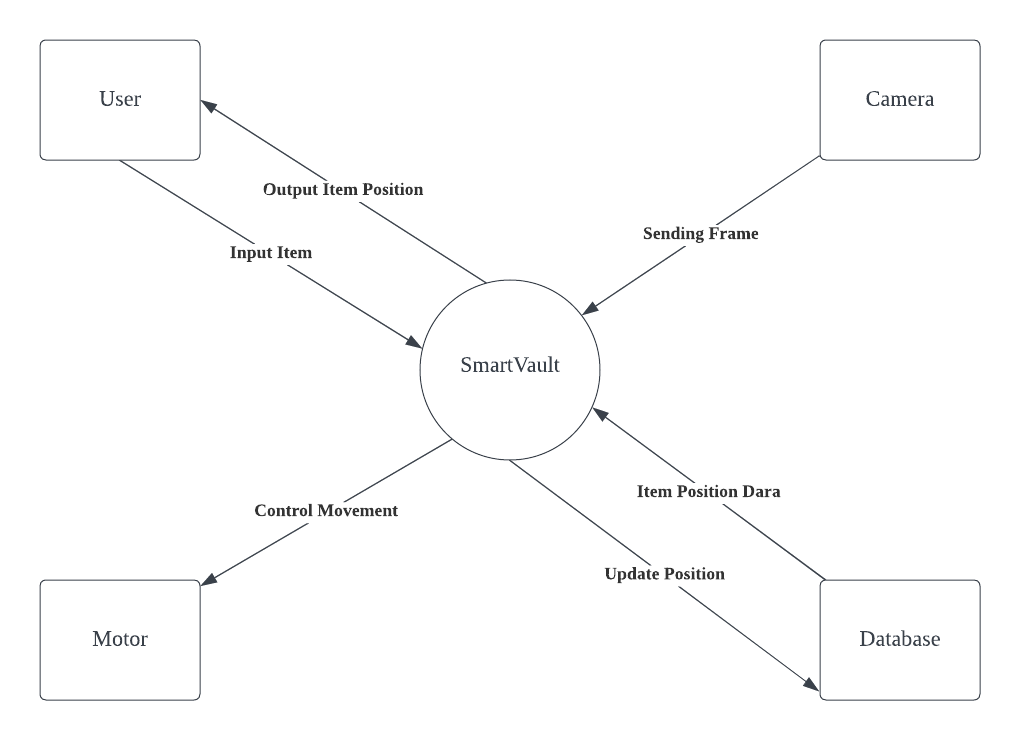
\includegraphics[scale=0.7]{Context.jpg}
    \caption{Context of Work}
\end{figure}
The following picture shows the design of the context diagram of the project, it illustrates the core interaction between the wheeled biped robot and its immediate external entities. In this diagram, the wheeled biped robot is the central system, the sensor sends inputs regarding the road condition and obstables, which acts as the external entity. The control system is another external entity that monitors the robot. The motor is used to drive the motion of the robot. This is consistent with what is described in the scope.


\section{Variables and Constants}

\subsection{Monitored and Controlled Variables (with units)}
\subsubsection{Monitored Variable}

\begin{table}[H]
\caption{Table of Monitored Variables} 
\begin{tabularx}{\textwidth}{XXXXX}
\toprule
\textbf{Variable Name} & \textbf{Type} & \textbf{Unit} & \textbf{Range} & \textbf{Comment} \\
\midrule
Battery Level & float & Ampere-hours (Ah) & Battery capacity & The remaining battery charge determines the operational time of the robot.\\\\
Motor temperature & float & Degree Celsius & motor's working temperature & Prevent overheating of the motor \\\\
Obstacle Proximity & Float & Meter & 0 to the dimension of the space & Measuring the distance to the nearby obstacles to prevent collisions \\\\
Terrain condition& Not applicable & Not applicable & Not applicable & Detect uneven or slippery terrain \\\\

\bottomrule
\end{tabularx}
\end{table}





\subsubsection{Controlled Variable}

\begin{table}[H]
\caption{Table of Control Variables} 
\begin{tabularx}{\textwidth}{XXXXX}
\toprule
\textbf{Variable Name} & \textbf{Type} & \textbf{Unit} & \textbf{Range} & \textbf{Comment} \\
\midrule
Robot's position & list of int & Meter & The dimension of the space for travel & Tracking position for navigation and path planning.\\\\
Robot's orientation& Not applicable & Not applicable & Either positive or negative & the direction that the robot moves\\\\
Robot's velocity &  Float &$m/s$ & Within the calculated safe range that is compatible with the motor's capacity.& The speed of the robot travels\\\\
Robot's acceleration &  Float & $m/s^2$& Within the calculated safe range and motor's capacity& The speed of the robot travels\\\\
Joint angles & Float & Radian & (0, 2$\pi$) & Monitor the angles of the leg joints to maintain the balance \\\\


\bottomrule
\end{tabularx}
\end{table}

\begin{table}[H]
\caption{Table of Control Variables (continued)} 
\begin{tabularx}{\textwidth}{XXXXX}
\toprule
\textbf{Variable Name} & \textbf{Type} & \textbf{Unit} & \textbf{Range} & \textbf{Comment} \\
\midrule
Torque of legs & Float & $Nm$ & The calculated range of torque within which the robot can operate normally.& Rotational force generated by the motor for completing tasks, such as jumping over the obstacles\\\\
Motor Voltage & Int & Volt & Based on required voltage that can support motion of the robot& Regulate the motor speed\\\\


\bottomrule
\end{tabularx}
\end{table}




\subsection{Constants}
\begin{table}[H]
\caption{Table of Constants} 
\begin{tabularx}{\textwidth}{XXXXX}
\toprule
\textbf{Variable Name} & \textbf{Type} & \textbf{Unit} & \textbf{Range} & \textbf{Comment} \\
\midrule
Mass of the robot& float& kg & The accepted calculated range & The robot should not be too light or too heavy, else, it may hinder its ability to perform tasks effectively\\\\
PID Controller Parameters& float& not applicable & not applicable& Gains should be adjusted to fine-tune motor response and control performance.\\\\
Physical dimensions& Set of floats & $cm$& within calculated accepted range& Height, width and length of the robot should be calculated and decided.
\\\\

\bottomrule
\end{tabularx}
\end{table}


\section{Behaviour}
\subsection{Behaviour Overview with Notation}
To make the behaviour of the product to achieve the target task, the Finite State Machine is created to describe the behaviour with detailed description provided after the picture. 
\begin{figure}[H]
    \centering
    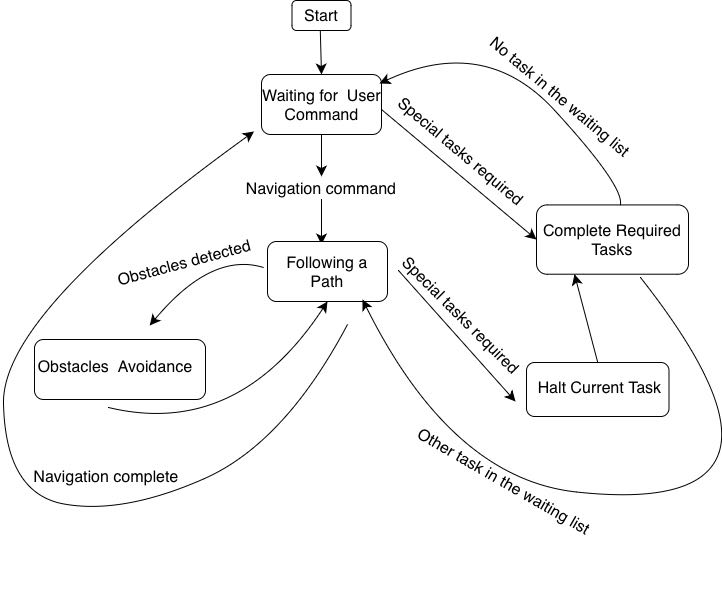
\includegraphics[scale=0.6]{FSM.jpg}
    \caption{The Picture of Finite  State Machine}
\end{figure}

\subsection{Brief Behaviour Description}
The FSM diagram briefly introduces the following general behaviours. The description is given below:\\\\
\noindent\textbf{Waiting for User Commands:} When the wheeled biped robot is positioned on the ground, in the absence of any initial user commands, it enters an "Idle" state. During this state, the robot's motor system is powered on, and the robot readies itself to receive and respond to user commands once they are initiated. \\\\
\noindent\textbf{Following a Path:} Upon receiving a navigation command, the robot initiates movement and begins the process of pathfinding to determine the most suitable route to follow.\\\\
\textbf{Obstacles Avoidance:}When the sensor detects nearby obstacles, it communicates this information to the control system. Subsequently, the control system takes action to navigate and bypass the obstacles to ensure the robot's safe passage.   \\\\
\textbf{Halt Current Task:} The system temporarily interrupts the ongoing path travel task and initiates the execution of a special task.\\\\
\textbf{Complete Required Tasks:} If special commands are issued while the robot is in motion, the robot promptly executes the specified tasks. These tasks may involve actions such as adjusting posture (e.g., lifting legs), changing direction (turning around), or performing dynamic movements like jumping. \\\\


\subsection{Required Behaviour Description and Rationales}
\subsection{Diagrams Showing Functional Decomposition}


% \begin{figure}[H]
%     \centering
%     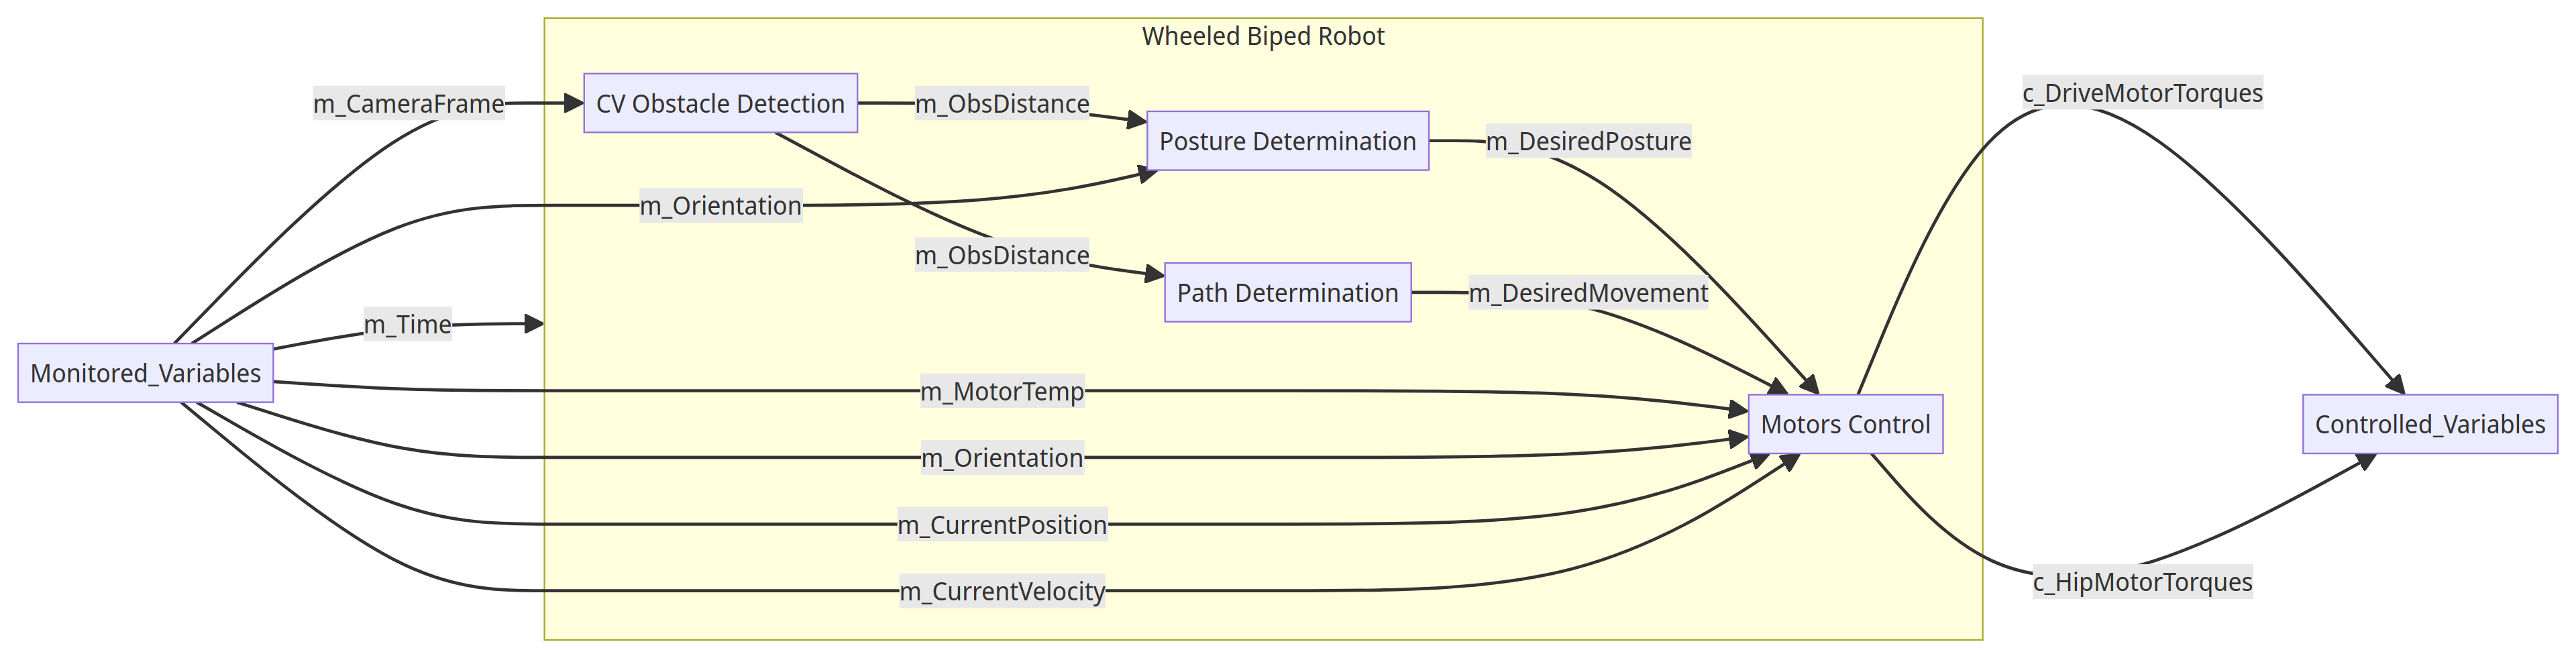
\includegraphics[scale=0.3]{Function_Decom.png}
%     \caption{Functional Decomposition Diagram}
% \end{figure}



\section{Requirements}



\subsection{Performance Requirements}
\subsubsection{Functional Requirements}
\textbf{Robot Mobility}\\\
\noindent\textbf{Seamless Movement:} The wheeled biped robot must be capable of moving smoothly and without jerky motions in various directions, including forward, backward, left, right, and rotation.\\\\
\noindent\textbf{Obstacle Handling:} The robot should be able to navigate through unpredictable environments with obstacles of varying sizes and shapes. It must avoid collisions and adapt its movements to the environment.\\\\
\noindent\textbf{Stability:} The robot should maintain stability while moving on uneven terrain and when transitioning between different types of surfaces, such as from smooth floors to rough terrain.\\\\
\noindent\textbf{Speed:} The robot's average speed should be at least [define a specific speed requirement] when navigating through typical indoor environments. The maximum speed for safety should not exceed the defined maximum speed.\\\\
\textbf{Sensing and Perception}\\\
\noindent\textbf{Obstacle Detection:} The robot must detect obstacles in its path using sensors, cameras, or other means. It should identify obstacles at least 3 meters before reaching them.\\\\
\noindent\textbf{Environmental Awareness:}  The robot should be able to perceive the environment, including the floor condition, changes in elevation, and surface irregularities, to adjust its movements accordingly.\\\\
\noindent\textbf{Object Recognition:} The robot should be able to recognize and differentiate between various objects in its environment, such as people, furniture, and other potential obstacles.\\\\
\textbf{Response and Adaptation}\\\
\noindent\textbf{Real-time Responsiveness:} The robot must respond to environmental changes and obstacles in real-time, adjusting its path and speed to avoid collisions or disturbances.\\\\
\noindent\textbf{Adaptive Behavior:} The robot should exhibit adaptive behavior, making decisions based on the type and size of obstacles, the terrain, and the robot's current state.\\
\subsubsection{Nonfunctional Requirements}
\textbf{Durability and Reliability}\\\
\noindent\textbf{Operating Time:} The robot should be capable of continuous operation for at least [define a specific duration] before requiring recharging or maintenance.\\\\
\noindent\textbf{Reliability:} The robot should be highly reliable, with a low probability of system failures or malfunctions during operation.\\\\
\noindent\textbf{Robustness:} The robot should be able to withstand minor collisions or impacts without sustaining significant damage that would impair its performance.\\\\
\textbf{Battery Life}\\\
\noindent\textbf{Battery Endurance:} The robot's onboard power source should provide sufficient energy for the robot to operate for at least 5 hours on a single charge.\\\\
\noindent\textbf{Recharge Time:} The time required for recharging the robot's batteries should not exceed 2 hours to minimize downtime.\\\\
\textbf{Communication}\\\
\noindent\textbf{Wireless Communication:} The robot should be capable of establishing and maintaining wireless communication with external systems for remote control and data transfer.\\\\
\textbf{Safety}\\\
\noindent\textbf{Emergency Stop:} The robot must have an emergency stop mechanism that can be activated to halt all movements in case of an imminent collision or other safety concerns.\\\\
\noindent\textbf{User Interaction:} The robot should have a user-friendly interface that allows for safe and intuitive interaction with operators, including starting and stopping the robot.\\\\
\noindent\textbf{Fall Protection:} The robot should be equipped with mechanisms or sensors to prevent falls or tipping over when navigating uneven or inclined terrain.\\\\
\textbf{Compliance}\\\
\noindent\textbf{Regulatory Requirements:} The robot's performance should comply with all relevant safety and regulatory standards for robotics in the intended operating environment.
\subsection{Normal Operation}
\noindent During normal operation, the wheeled biped robot should execute its primary functions while adhering to the defined performance requirements. The following steps outline the typical sequence of actions and behaviors expected during normal operation:\\\\
\noindent\textbf{1. Start-up}\\
\noindent 1.1. The operator initiates the robot's start-up process using the user-friendly interface.\\
1.2. The robot performs a self-check to ensure all systems are functioning correctly.\\\\
\noindent\textbf{2. Localization and Mapping}\\
\noindent 2.1. The robot utilizes its sensors and cameras to create a map of the environment.\\
2.2. It identifies its current position and orientation within the environment.\\\\
\noindent\textbf{3. Path Planning}\\
\noindent 3.1. Based on the map and sensor data, the robot generates a path to its target destination.\\
3.2. It considers obstacles, terrain conditions, and environmental factors during path planning.\\\\
\noindent\textbf{4. Movement}\\
\noindent 4.1. The robot smoothly and seamlessly moves towards its destination, following the planned path.\\
4.2. It continuously monitors its surroundings to detect obstacles, changes in terrain, or potential safety concerns.\\
4.3. The robot adapts its movements in real-time to avoid collisions and ensure stability.\\\\
\noindent\textbf{5. Sensing and Perception}\\
\noindent 5.1. The robot continually scans its environment to detect obstacles and changes in the surroundings.\\
5.2. It recognizes and classifies objects, including people and obstacles.\\
5.3. The robot updates its map and path as necessary based on new information.\\\\
\noindent\textbf{6. Communication}\\
\noindent 6.1. The robot maintains wireless communication with external systems, allowing for remote control and data exchange.\\
6.2. It transmits sensor data and receives control commands as needed.\\\\
\noindent\textbf{7. Safety}\\
\noindent 7.1. The robot's safety mechanisms are actively engaged throughout normal operation.\\
7.2. If an imminent collision is detected, the emergency stop mechanism is triggered, bringing the robot to a halt.\\
7.3. Fall protection mechanisms prevent tipping or falling on uneven terrain.\\\\
\noindent\textbf{8. Battery Management}\\
\noindent 8.1. The robot monitors its battery levels to ensure it has sufficient power for the intended operation duration.\\
8.2. When the battery level is low, the robot autonomously returns to a designated charging station for recharging.\\
8.3. Recharge time is optimized to minimize downtime.\\\\
\noindent\textbf{9. User Interaction}\\
\noindent 9.1. Operators can interact with the robot through the user-friendly interface.\\
9.2. They can issue commands, check the robot's status, and stop or resume its operation as needed.\\\\
\noindent\textbf{10. Compliance}\\
\noindent 10.1. The robot operates in compliance with all relevant safety and regulatory standards for its operating environment.
\subsection{Undesired Event Handling}
\noindent In the event of unforeseen or undesired situations during the operation of the wheeled biped robot, the system should have mechanisms in place to handle such events safely and effectively. This section outlines how the robot should respond to various undesired events and conditions:\\\\
\noindent\textbf{1. Collision or Obstacle Blocking}\\
\noindent 1.1. When the robot detects an obstacle in its path or experiences a collision, it should immediately initiate an emergency stop.\\
1.2. The robot should backtrack or re-plan its path to navigate around the obstacle and resume its mission once the path is clear.\\\\
\noindent\textbf{2. Loss of Communication}\\
\noindent 2.1. If the robot loses wireless communication with external systems or operators, it should attempt to re-establish the connection.\\
2.2. If communication cannot be re-established within a predefined time frame, the robot should follow a predefined safe protocol, which may include stopping or returning to a designated safe location.\\\\
\noindent\textbf{3. Battery Depletion}\\
\noindent 3.1. When the robot's battery level reaches a critical threshold, it should autonomously navigate to a designated charging station to recharge.\\
3.2. If the robot cannot reach the charging station, it should engage its emergency stop mechanism to prevent complete battery depletion.\\\\
\noindent\textbf{4. System Faults}\\
\noindent 4.1. In the event of a system fault or malfunction, the robot should log the error and take appropriate actions to ensure safe operation.\\
4.2. If the fault is critical and impacts safety or functionality, the robot should initiate an emergency stop and alert operators.\\\\
\noindent\textbf{5. Environmental Extremes}\\
\noindent 5.1. If the robot encounters extreme environmental conditions such as heavy rain, extreme temperatures, or adverse terrain, it should adjust its operation to minimize risk.\\
5.2. The robot should prioritize safety over mission completion in such conditions.\\\\
\noindent\textbf{6. Loss of Localization}\\
\noindent 6.1. If the robot loses its localization or mapping capabilities, it should attempt to re-establish its position within the environment.\\
6.2. If re-localization is not possible, the robot should stop to avoid unpredictable behavior.\\\\
\noindent\textbf{7. Human Interference}\\
\noindent 7.1. The robot should be designed to respond safely to unexpected human interference, such as attempts to obstruct its path or physical interactions.\\
7.2. It should avoid collisions with humans while maintaining its primary mission.\\\\
\noindent\textbf{8. Emergency Situations}\\
\noindent 8.1. In case of emergency, the robot should have an accessible manual override mechanism that can be used by operators to take control and ensure safety.\\
8.2. Operators should be able to trigger an emergency stop remotely.\\\\
\noindent\textbf{9. Logging and Reporting}\\
\noindent 9.1. The robot should log all significant events and responses, including undesired events and system faults.\\
9.2. It should provide a mechanism for reporting these events to operators or maintenance personnel for analysis and troubleshooting.
\subsection{Likelihood of Change in Requirements}
\noindent During the development of the wheeled biped robot, it is important to acknowledge that some requirements may be more susceptible to change than others due to evolving technology, changing project constraints, or evolving stakeholder needs. This section categorizes the requirements into two lists: those likely to change and those unlikely to change.
    \subsubsection{List of Requirements likely to Change}
    \noindent\textbf{Speed: }The specified average speed may need adjustment as technology advancements allow for improved mobility.\\\\
    \noindent\textbf{Battery Endurance: }As battery technology evolves, the robot's expected operating time may increase.\\\\
    \noindent\textbf{Safety: }Regulatory requirements for safety may change over time, requiring updates to safety mechanisms.\\\\
    \noindent\textbf{Compliance: }Regulatory standards and compliance requirements may change due to new industry regulations.
    \subsubsection{List of Requirements unlikely to Change}
    \noindent\textbf{Seamless Movement: }The fundamental requirement for smooth and seamless movement is unlikely to change, as it is a core performance requirement.\\\\
    \noindent\textbf{Obstacle Detection: }The need for the robot to detect obstacles remains constant to ensure safe navigation.\\\\
    \noindent\textbf{Emergency Stop: } The requirement for an emergency stop mechanism will remain a critical safety feature.\\\\
    \noindent\textbf{User Interaction: } The need for a user-friendly interface to interact with the robot is a fundamental requirement.\\\\
    \noindent\textbf{Loss of Communication: }The response to a loss of communication remains vital to maintain control and safety.

\newpage
\section{Reference}

\end{document}
